% !TeX encoding = UTF-8 Unicode
\documentclass[a4paper,12pt]{article}
\usepackage[english]{babel}
\usepackage[english]{isodate}
\usepackage{graphicx}
\usepackage{hyperref}
\usepackage{centernot}
\usepackage{xfrac}
\usepackage{mathtools}
\usepackage{enumitem}
\usepackage{fancyhdr}
\usepackage{lastpage}
\usepackage{xcolor}
\usepackage{changepage}
\usepackage{amsthm}
\usepackage{amsfonts}
\usepackage{amsmath}
\usepackage{amssymb}
\usepackage{soul}
\usepackage{float}
\usepackage{centernot}
\usepackage{tcolorbox}
\usepackage{titling}
\usepackage{caption}
\usepackage{subcaption}
\usepackage{etoolbox}
\usepackage{listings}
\usepackage{biblatex}
\usepackage{csquotes}
\usepackage{titlesec}
\usepackage{tikz}
\usetikzlibrary{trees}

\addbibresource{bibliography.bib}

\patchcmd{\section}{\bfseries}{\bfseries\boldmath }{}{}
\patchcmd{\subsection}{\bfseries}{\bfseries\boldmath }{}{}
\patchcmd{\subsubsection}{\bfseries}{\bfseries\boldmath }{}{}

\hypersetup{
  colorlinks=True,
  urlcolor=blue,
  citecolor=red,
  menucolor=black,
}

\renewcommand{\UrlFont}{\ttfamily\footnotesize}

\lstdefinelanguage{futhark}
{
  % list of keywords
  morekeywords={
  do,
  else,
  for,
  if,
  in,
  include,
  let,
  loop,
  then,
  type,
  val,
  while,
  with,
  module,
  def,
  entry,
  local,
  open,
  import,
  assert,
  match,
  case,
  },
  sensitive=true, % Keywords are case sensitive.
  morecomment=[l]{--}, % l is for line comment.
  morestring=[b]" % Strings are enclosed in double quotes.
}


\lstset{
  language=futhark,
  showspaces=false,
  showstringspaces=false,
  mathescape=true,
  aboveskip=0pt,
  belowskip=6pt,
  numberstyle=\tiny,
  numbers=left, 
  firstnumber=1,
  numberfirstline=true,
  tabsize=4,
  breaklines=true,
}

\newcommand\LAST{\text{LAST}}
\newcommand\defiff{\mathrel{\stackrel{\makebox[0pt]{\mbox{\normalfont\tiny def}}}{\iff}}}
\newcommand\defeq{\mathrel{\stackrel{\makebox[0pt]{\mbox{\normalfont\tiny def}}}{=}}}
\newcommand\concat{\: \mathrlap{+} \: +}
\newcommand\map{\textbf{map}\ }
\newcommand\reduce{\textbf{reduce}\ }
\theoremstyle{definition}
\newtheorem{definition}{Definition}[section]
\newtheorem{proposition}{Proposition}[section]
\newtheorem{corollary}{Corollary}[section]
\newtheorem*{remark}{Remark}
\newtheorem{lemma}{Lemma}[section]
\newtheorem{theorem}{Theorem}
\newtheorem{algorithm}{Algorithm}[section]
\newtheorem{example}{Example}[section]
\newtheorem{conjecture}{Conjecture}[section]
\DeclareMathOperator{\sign}{sign}
\newcommand\doubleplus{+\kern-1.3ex+\kern0.8ex}
\newcommand\mdoubleplus{\ensuremath{\mathbin{+\mkern-10mu+}}}

\newcommand{\id}[1]{\ensuremath{\mathit{#1}}}
\newcommand{\kw}[1]{\ensuremath{\mathtt{#1}}}
\newcommand{\Let}{\kw{let}}
\newcommand{\In}{\kw{in}}
\newcommand{\If}{\kw{if}}
\newcommand{\Then}{\kw{then}}
\newcommand{\Else}{\kw{else}}
\newcommand{\Filter}{\kw{filter}}
\newcommand{\Or}{\kw{or}}
\newcommand{\Groupby}{\kw{groupby}}
\newcommand{\Partition}{\kw{partition}}
\newcommand{\Scatter}{\kw{scatter}}
\newcommand{\Hist}{\kw{hist}}
\newcommand{\Map}{\kw{map}}
\newcommand{\Sum}{\kw{sum}}
\newcommand{\Mod}{\kw{mod}}
\newcommand{\Fst}{\kw{fst}}
\newcommand{\Snd}{\kw{snd}}
\newcommand{\Presum}{\kw{presum}}
\newcommand{\True}{\kw{true}}
\newcommand{\False}{\kw{false}}
\newcommand{\Sort}{\kw{sort}}
\newcommand{\Segor}{\kw{segor}}
\newcommand{\Hash}{\kw{hash}}
\newcommand{\Random}{\kw{random}}
\newcommand{\Iota}{\kw{iota}}
\newcommand{\Unzip}{\kw{unzip}}
\newcommand{\Unit}{\mathbf{unit}}
\newcommand{\Int}{\mathbf{int}}
\newcommand{\Bool}{\mathbf{bool}}
\newcommand{\Def}{\kw{def}}
\newcommand{\Rep}{\kw{rep}}
\newcommand{\Zip}{\kw{zip}}

\fancyhf{}
\setlength{\headheight}{14.49998pt}
\pretitle{\vspace{-120pt}\begin{center}}
\posttitle{\par\end{center}\vspace{-80pt}}
\fancyhead[C]{}
\fancyfoot[R]{Page \thepage \hspace{1pt} of \pageref{LastPage}}
\pagestyle{fancy}
\fancypagestyle{firstpage}{%
  \fancyhf{}
  \renewcommand{\headrulewidth}{0pt}
  \fancyfoot[R]{Page \thepage \hspace{1pt} of \pageref{LastPage}}
}
\title{
  {\Large \textsc{University of Copenhagen}} \\[5pt]
  {\large Data-Parallel Union-Find} \\[10pt]
  Author: William Henrich Due \\[0pt]
}
\author{}
\date{}

\begin{document}
\maketitle
\thispagestyle{firstpage}

\section{Theory}
This section will derive the theoretical foundation for the data-parallel
union-find. The theory is based on set theory, graph theory and properties of
forests.
\subsection{Forests}
To be able to define a union-find structure we first need to define some basic
graph theory and specifically in relation to forests. The graphs used are
directed graphs $G = (V, E)$ where $V$ is a set of vertices and $E
\subseteq V \times V$ is a set of directed edges. Initially we need a definition
of what it means for node $u \in V$ to be reachable from node $v \in V$ meaning
there is a path from $u$ to $v$.

\begin{definition}[Reachability]
  A node $v$ is \emph{reachable} from a node $u$ in a directed graph $G = (V,
  E)$ if there exists a sequence of directed edges $e_1, e_2, \ldots, e_m \in
  E$ where $m \geq 1$ and $e_i = (v_{i-1}, v_i)$ for $1 \leq i \leq m$,
  such that $v_0 = u$ and $v_m = v$. We denote this by $u \leadsto v$.
\end{definition}
\noindent One of the first properties of reachability is it is neither
\text{reflexive} nor \textit{irreflexive}. The reason for chosing such a
definition is that the definition of an cycle in a directed graph becomes
simply.
\begin{definition}[Cycle]
  A cycle in a directed graph $G = (V, E)$ has a cycle if there exists
  $v \in V$ such that $v \leadsto v$.
\end{definition}
\noindent With this definition of cycles a forest can be defined as follows:
\begin{definition}[Forest]
  A forest is a directed graph $F = (V, E)$ where $V$ is a set of vertices and $E
  \subseteq V \times V$ is a set of directed edges such that:
  \begin{enumerate}
    \item There are no cycles $v \centernot\leadsto v$ for all $v \in V$, and
    \item each node has at most one parent i.e. for all $(u, v_1), (u, v_2)
    \in E$ it holds that $v_1 = v_2$.
  \end{enumerate}
\end{definition}
\noindent With the definition of a forest we can now define roots in a forest.
\begin{definition}[Root]
  A node $v \in V$ in a forest $F = (V, E)$ is a root if it has no parent.
  This is defined as the predicate:
  \begin{align*}
    \mathcal{R}_F(v) : v \centernot\leadsto u \text{ for all } u \in V
  \end{align*}
\end{definition}
\noindent Using the definition of a root we can now define a tree as a special
case of a forest.
\begin{definition}[Tree]
  A tree is a forest $T = (V, E)$ where there exists a unique root $r \in V$
  such that $v \leadsto r$ for all $v \in V\backslash
  \{r\}$.
\end{definition}
\noindent Futhermore we will now work towards seeing a forest as a collection of
trees. To do this we first need to establish how many roots a forest has.
\begin{proposition}[Forest Root Count]\label{prop:forest-root-count}
    A forest $F = (V, E)$ where $|V| = n$ and $|E| = n - k$ has $k$ roots.
\end{proposition}

\begin{proof}
    Let $F = (V, E)$ be a forest where $|V| = n$ and $|E| = n - k$. By the
    second property of a forest then $n - k$ vertices must have a parent. Since
    there are $n$ vertices in total it follows that there are exactly $k$
    vertices $r_1, r_2, \ldots, r_k \in V$ that has no parent. Hence there are
    exactly $k$ roots in $F$.
\end{proof}
\noindent Knowing how many roots a forest does not finish the picture of how
a forest is a collection of trees. We also need to show that each vertex also
has a path to a root.
\begin{proposition}[Root Path Exist]\label{prop:roots-path-exist}
  In a forest $F = (V, E)$ for each element $v \in V$ there exists a root $r \in
  V$ such that $\mathcal{R}_F(r)$ and either $v \leadsto r$ or $v = r$.
\end{proposition}

\begin{proof}
  Let $F = (V, E)$ be a forest and $v \in V$ be an arbitrary element in $V$. By
  proposition \ref{prop:forest-root-count} there exists at least one root $r \in
  V$ such that $\mathcal{R}_F(r)$. This can be shown by structural induction on
  a vertex $v \in V$ that either $v = r$ or $(v, p) \in E$ such that $p \leadsto
  r$.
  \begin{itemize}
    \item If $(v, p) \notin E$ then $v \centernot\leadsto u \text{ for all } u \in V$ so $v = r$.
    \item If $(v, p) \in E$ then by induction hypothesis $p \leadsto r$ such
    that $r \in V$ and $\mathcal{R}_F(r)$. It follows that since $v \leadsto p
    \leadsto r$ so $v \leadsto r$.
  \end{itemize}
\end{proof}
\noindent Lastly we can finish the picture of a forest being a collection of
trees by showing that the path from a vertex to a root is unique. So that there
is only one tree for each vertex in the forest.
\begin{proposition}[Unique Path]\label{prop:unique-path}
  Let $F = (V, E)$ be a forest and $v, u \in V$. If $v \leadsto u$ then the path
  from $v$ to $u$ is unique.
\end{proposition}
\begin{proof}
  Let $F = (V, E)$ be a forest, $v, u \in V$ and $v \leadsto u$. Since every
  vertex has at most one parent by the second property of a forest it follows
  that there is only one out going edge from each vertex in the path from $v$ to
  $u$. Hence the path from $v$ to $u$ is unique.
\end{proof}

% \begin{proposition}[Forest Edge Limit]\label{prop:forest-edge-limit}
%   A forest $F = (V, E)$ where $|V| = n$ and $|E| > n - 1$ is not a forest.
% \end{proposition}
% 
% \begin{proof}
%   Let $F = (V, E)$ be a forest where $|V| = n$ and $|E| > n - 1$. By
%   proposition \ref{prop:forest-root-count} a forest with $n - 1$ has exactly
%   one root, so it is a tree. By adding one more edge to the tree it must make
%   one vertex have two parents. Or since every vertex $v \in V$ has a path to
%   the root $r \in V$ it must create a cycle $v \leadsto v$ for some $v \in V$.
%   In both cases it contradicts the properties of a forest.
% \end{proof}

\subsection{Union-Find Structure}
Using the definition of a forest we can now define a union-find structure, the
way it will represented is as a forest. Here the forest represents an
equivalence on $V$ where each tree in the forest represents an equivalence
class.
\begin{definition}[Union-Find Structure]
  A union-find structure is a forest $F = (V, E)$.
\end{definition}
\noindent The way this equivalence relation is defined is by the representative
of each element in the forest. The representative of a node is found by
traversing the edges in the forest until a root is found. Using the notion of a
root we can now define the representative of an element in a forest.
\begin{definition}[Representative]
  The representative of an element $v \in V$ in a forest $F = (V, E)$ is the
  root $r \in V$ such that there is a path from $v$ to $r$. This is defined as
  the function:
  \begin{align*}
    \rho_F(v) := r \text{ where } r \in V \text{ such that } \mathcal{R}_F(r) \land (v \leadsto r \lor v = r)
  \end{align*}
\end{definition}
\noindent With the notion of a representative it is possible to define the set
of vertices in the same tree in a forest.
\begin{definition}[Tree Set]
  The set of vertices of the same tree $\mathcal{E}_F(v)$ in a
  forest $F = (V, E)$ is defined as:
  \begin{align*}
    \mathcal{E}_F(v) := \{u : u \in V \text{ where } \rho_F(u) = \rho_F(v)\}
  \end{align*}
\end{definition}
\noindent The notion of equivalence classes can now be formalized using the the
definition of a partition. We need this to show properties of the union-find
structure.
\begin{definition}[Partition]\label{def:partition}
  The set $P \subseteq \mathbb{P}(S)$ is a partition of a set $S$ if:
  \begin{enumerate}
    \item $a \neq \emptyset$ for all $a \in P$
    \item $a \cap b = \emptyset$ for all $a, b \in P$ where $a
    \neq b$
    \item $\bigcup_{a \in P} a = S$
  \end{enumerate}
  We say that $P$ is a partition of $S$ and $P$ forms an equivalence relation on
  $S$ where each $a \in P$ is an equivalence class.
\end{definition}
\noindent Using the definition of a partition we can now show that a forest is a
partition of its vertices based on the tree sets.
\begin{proposition}[Forest Partition]\label{prop:forest-partition}
  A forest $F = (V, E)$ is a partition of $V$ for the following set:
  \begin{align*}
    \{\mathcal{E}_F(v) : v \in V\}
  \end{align*}
\end{proposition}

\begin{proof}
  Let $F = (V, E)$ be a forest. We will show that the set in the proposition
  is a partition of $V$ by showing that it satisfies the three properties in
  definition \ref{def:partition}.
  \begin{enumerate}
    \item By definition of $\mathcal{E}_F(v)$ it can not be empty since for
    $\mathcal{E}_F(v)$ then $\rho_F(v) = \rho_F(v)$. Hence $\mathcal{E}_F(v)
    \neq \emptyset$ for all $v \in V$.
    \item Let $a$ and $b$ be two arbitrary elements in the set such that $a
    \neq b$. By definition of $a$ and $b$ there exists $v_1, v_2 \in V$ such
    that $a = \{u : u \in V \land \rho_F(u) = \rho_F(v_1)\}$ and $b = \{u :
    u \in V \land \rho_F(u) = \rho_F(v_2)\}$. Since $a \neq b$ it follows
    that $\rho_F(v_1) \neq \rho_F(v_2)$ since otherwise $a = b$, hence $a
    \cap b = \emptyset$.
    \item Let $v$ be an arbitrary element in $V$. By proposition
    \ref{prop:roots-path-exist} there exists a root $r \in V$ such that
    $\mathcal{R}_F(r)$ and $v \leadsto r$ or $v = r$. By definition of the
    representative it follows that $\rho_F(v) = r$. Now let $a = \{u : u \in
    V \land \rho_F(u) = \rho_F(v)\}$. By definition of $a$ it follows that
    $v \in a$. Since $v$ was arbitrary it follows that $\bigcup_{a \in P} a
    = V$.
  \end{enumerate}
\end{proof}
\noindent With the notion of a partition of a forest we can now define the equivalence relation on the forest.
\begin{definition}[Same Tree Relation]
  The relation $\sim_F$ on a forest $F$ is defined as:
  \begin{align*}
    u \sim_F v :\iff u \in \mathcal{E}_F(v)
  \end{align*}
\end{definition}
\noindent Trivially we can now show that the same tree relation is an
equivalence relation.
\begin{corollary}[Same Tree Relation is an Equivalence Relation]
  The relation $\sim_F$ on a forest $F$ is an equivalence relation due to
  $\{\mathcal{E}_F(v) : v \in V\}$ being a partition of $V$.
\end{corollary}

\begin{proof}
   From proposition \ref{prop:forest-partition} we directly get that $(V,
    \sim_F)$ is an equivalence relation since the set $\{\mathcal{E}_F(v) : v
    \in V\}$ is a partition of $V$.
\end{proof}
\noindent Now using the notion of partitions we can determine if two forests
are equivalent in the sense that they have the same tree sets. This is useful
when showing that two union-find structures are equivalent.

\begin{definition}[Forests with Equivalent Tree Sets]
  Two forests $F = (V, E)$ and $F' = (V', E')$ have equivalent tree sets $F
  \cong F'$ if:
  \begin{itemize}
    \item Vertices are the same $V = V'$.
    \item The tree sets are equivalent $\mathcal{E}_{F}(v) =
    \mathcal{E'}_F(v)$ for all $v \in V$.
  \end{itemize}
\end{definition}
\noindent It is also possible to define the property of uniting two trees in a
forest should satisfy. We would want the resulting forest to have that the two
trees are now one tree containing all the elements from both trees. And all
other trees in the forest should remain unchanged.
\begin{definition}[Tree Union Property]\label{def:tree-union-property}
  The tree union of two elements $v$ and $u$ for a forest $F = (V, E)$ is such
  that $v \sim_{F'} u$ in a new forest $F' = (V', E')$ and $F'$ satify the
  following properties:
  \begin{enumerate}
    \item $\mathcal{E}_{F'}(v) = \mathcal{E}_{F'}(u) = \mathcal{E}_F(v) \cup \mathcal{E}_F(u)$ and
    \item $\mathcal{E}_{F'}(w) = \mathcal{E}_F(w) \text{ for all } w \in V
    \backslash (\mathcal{E}_F(v) \cup \mathcal{E}_F(u))$.
  \end{enumerate}
\end{definition}
\noindent It is now possible to define a tree union operation that satisfies the
tree union property. It uses the fact that if we make the representative of one
tree the parent of the representative of the other tree then all elements in the
two trees will have the same representative in the new forest. But we actually
only care about the trees still being trees and not the structure of the trees
themselves. Hence it does not matter which representative becomes the parent of
the other.
\begin{proposition}[Root Union]\label{prop:root-union}
  Let forest $F = (V, E)$, $p = \rho_F(u)$ be the representative of $u$ and
  let $q = \rho_F(v)$ be the representative of $v$ where $q \neq p$. Then
  define $F'$ as:
  \begin{align*}
    F' &:= (V, E \cup \{(q, p)\})
  \end{align*}
  Then $u \sim_{F'} v$ in $F'$ and $F'$ will satisfy the properties of a tree
  union.
\end{proposition}

\begin{proof}
  Let $F = (V, E)$, $p = \rho_F(u)$ be the representative of $u$ and let $q =
  \rho_F(v)$ be the representative of $v$. By definition $q$ will have parent
  $p$ in $F'$ and since $q$ is a root it has no parent then $F'$ is a forest.
  Now for all $w \in \mathcal{E}_F(q)$ it holds that $w \leadsto q$ or $q = w$
  and since $q \leadsto p$ it follows that $w \leadsto p$. Hence $w \in
  \mathcal{E}_{F'}(p)$ for all $w \in \mathcal{E}_F(q)$ and trivially $w \in
  \mathcal{E}_{F'}(p)$ for all $w \in \mathcal{E}_F(p)$ so it follows that
  $\mathcal{E}_{F'}(v) = \mathcal{E}_{F'}(u) = \mathcal{E}_F(v) \cup
  \mathcal{E}_F(u)$. Now let $w \in V \backslash (\mathcal{E}_F(v) \cup
  \mathcal{E}_F(u))$ be an arbitrary element. Since $w \centernot\leadsto p$,
  $w \neq p$, $w \centernot\leadsto q$, and $w \neq q$ it follows that $w$ has
  the same representative in $F'$ as in $F$ hence $\mathcal{E}_{F'}(w) =
  \mathcal{E}_F(w)$.
\end{proof}
This operation can now be used to define the union operation on a union-find
structure. This operation corresponds to the union operation in a trivial
sequential union-find data structure. The efficient implementations of
union-find will do things like path compression or path halving to optimize the
distance from a node to its representative. And these operations would also
fulfill the tree union property since they do not change the equivalence classes
of the forest. 

\subsection{Conflict-Free Sets}
The problem now is how to define a parallel union operation on a union-find
structure. The challenge is that multiple union operations might try to change
the same part of the forest at the same time. And do to the nature of working in
a data-parallel model we can not have atomic operations that would solve these
problems in an concurrent manner. The way this problem will be solve is we
consider a set of pairs of vertices that must be unified in the forest. We can
find the representative of all of these vertex pairs, these representative pairs
forms an graph of roots in the forest. We can simply pick out a subset of edges
from this graph of roots that forms a forest and glue these edges onto the
original forest. This will ensure that there are no conflicts when adding the
edges to the original forest. We will call such a set of edges a conflict-free
set. An example of a conflict-set is Root Union \ref{prop:root-union} since it
only adds one edge between two roots to the forest and hence there can not be
any conflicts.

An example of this process can be seen in figures \ref{fig:forest} here we have
a forest with three trees. In figure \ref{fig:conflict-free-set} we see the
graph of roots on the left and on the right a conflict-free set highlighted in
red. Finally in figure \ref{fig:forest-after-conflict-free} we see the resulting
forest after adding the conflict-free set to the original forest.
\begin{figure}[H]
    \centering  
    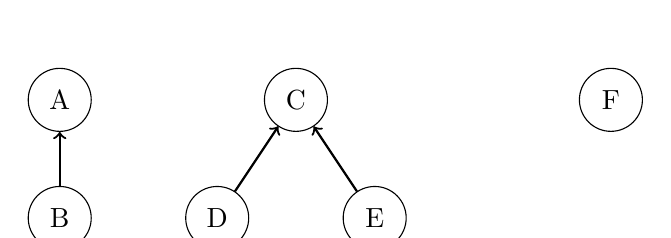
\begin{tikzpicture}[
        level distance=1.5cm,
        level 1/.style={sibling distance=2cm},
        every node/.style={circle, draw, minimum size=0.8cm}
    ]
    
    % First tree (A with child B)
    \node (A) at (0,0) {A}
        child {node (B) {B}};
    
    % Second tree (C with children D and E)
    \node (C) at (3,0) {C}
        child {node (D) {D}}
        child {node (E) {E}};
    
    % Third tree (just F)
    \node (F) at (7,0) {F};
    
    % Arrows from children to parent roots
    \draw[->, thick] (B) -- (A);
    \draw[->, thick] (D) -- (C);
    \draw[->, thick] (E) -- (C);
    
    \end{tikzpicture}
    \caption{A forest where there are three trees with representatives A, C and
    F.}
    \label{fig:forest}
\end{figure}

\begin{figure}[H]
    \centering  
    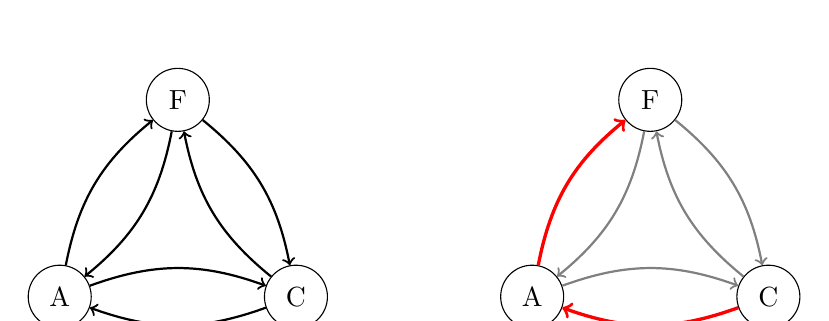
\begin{tikzpicture}[
        every node/.style={circle, draw, minimum size=0.8cm},
        every edge/.style={draw, ->, thick}
    ]
    
    % First graph
    \begin{scope}
        % Position the three nodes in a triangle
        \node (A) at (0,0) {A};
        \node (C) at (3,0) {C};
        \node (F) at (1.5,2.5) {F};
        
        % Create cycles with arrows
        \draw[->, thick] (A) to[bend left=20] (C);
        \draw[->, thick] (C) to[bend left=20] (A);
        
        \draw[->, thick] (C) to[bend left=20] (F);
        \draw[->, thick] (F) to[bend left=20] (C);
        
        \draw[->, thick] (F) to[bend left=20] (A);
        \draw[->, thick] (A) to[bend left=20] (F);
    \end{scope}
    
    % Second graph (shifted to the right with highlighted arrows)
    \begin{scope}[xshift=6cm]
        % Position the three nodes in a triangle
        \node (A2) at (0,0) {A};
        \node (C2) at (3,0) {C};
        \node (F2) at (1.5,2.5) {F};
        
        % Create cycles with arrows (normal)
        \draw[->, thick, gray] (A2) to[bend left=20] (C2);
        \draw[->, thick, red, very thick] (C2) to[bend left=20] (A2);  % Highlighted C -> A
        
        \draw[->, thick, gray] (C2) to[bend left=20] (F2);
        \draw[->, thick, gray] (F2) to[bend left=20] (C2);
        
        \draw[->, thick, gray] (F2) to[bend left=20] (A2);
        \draw[->, thick, red, very thick] (A2) to[bend left=20] (F2);  % Highlighted A -> F
    \end{scope}
    
    \end{tikzpicture}
    \caption{On the left a graph of roots from Figure \ref{fig:forest}. On the right a conflict-free set highlighted in red.}
    \label{fig:conflict-free-set}
\end{figure}

\begin{figure}[H]
    \centering  
    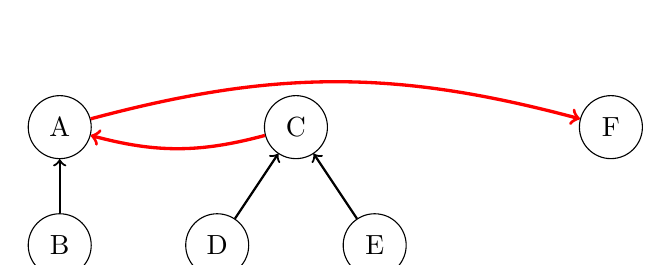
\begin{tikzpicture}[
        level distance=1.5cm,
        level 1/.style={sibling distance=2cm},
        every node/.style={circle, draw, minimum size=0.8cm}
    ]
    
    % First tree (A with child B)
    \node (A) at (0,0) {A}
        child {node (B) {B}};
    
    % Second tree (C with children D and E)
    \node (C) at (3,0) {C}
        child {node (D) {D}}
        child {node (E) {E}};
    
    % Third tree (just F)
    \node (F) at (7,0) {F};
    
    % Original arrows from children to parent roots
    \draw[->, thick] (B) -- (A);
    \draw[->, thick] (D) -- (C);
    \draw[->, thick] (E) -- (C);
    
    % New highlighted edges
    \draw[->, very thick, red] (A) to[bend left=15] (F);
    \draw[->, very thick, red] (C) to[bend left=15] (A);
    
    \end{tikzpicture}
    \caption{The forest from Figure \ref{fig:forest} after adding the
    conflict-free set from Figure \ref{fig:conflict-free-set}.}
    \label{fig:forest-after-conflict-free}
\end{figure}
\noindent The formal definition of a conflict-free set is as previous described
a set of root pairs that forms a forest.
\begin{definition}[Conflict-free Set]
  Let $F$ be a forest, $X \subseteq \{(\rho_F(v), \rho_F(u)) : (v, u) \in V
  \times V\}$ be a set of root pairs. Then $X$ is a conflict-free set in $F$
  if $(V, Y)$ is a forest.
\end{definition}
\noindent With this definition of a conflict-free set we now wish to show that
we can add all edges in a conflict-free set to a forest and still have a forest.
\begin{proposition}[Conflict-free Forest Union]\label{prop:conflict-free-forest-union}
  Let forest $F = (V, E)$ be a forest and let $X \subseteq V \times V$ be a
  conflict-free set in $F$ where $|X| = n$. Then defining the following forests:
  \begin{align*}
    F_0 &:= F \\
    F_{i} &:= (V, E_{i - 1} \cup \{(v_i, u_i)\}) \text{ for } (v_i, u_i) \in X \text{ and } 1 \leq i \leq n
  \end{align*}
  Then $F_n$ is a forest.
\end{proposition}

\begin{proof}
  Let forest $F = (V, E)$ be a forest, $X \subseteq V \times V$ be a
  conflict-free set in $F$. We will show that $F_n$ is a forest by induction
  on $i$.
  \begin{itemize}
    \item Base case: If $i = 0$ then $F_i = F_0 = F$ which is a forest.
    \item Induction hypothesis: Assume that $F_{i - 1}$ is a forest for all
    $1 \leq i < n$.  Let $(v_i, u_i) \in X$, we know that $v_i \neq v_j$ for
    all $(v_j, u_j) \in Y \backslash \{(v_i, u_i)\}$ since otherwise $(V,
    X)$ would not be a forest and $X$ would not be a conflict-free set in
    $F$. So $v_i$ will only have one parent in $F_i$ since it only appears
    once as a child in $(V, X)$. By definition all of the edges in $X$
    consists of roots in $F$, and since $(V, X)$ is a forest there are no
    cycles $y \centernot\leadsto y$ for all $y \in V$ in $F_i$. Hence $F_i$
    is a forest.
  \end{itemize}
  Thus by induction $F_n$ is a forest.
\end{proof}
\noindent We also need to show that Conflict-free Forest Union
\ref{prop:conflict-free-forest-union} satisfies Tree Union Property
\ref{def:tree-union-property}. This is done by showing that adding edges from
the conflict-free set to a forest in any order is equivalent to adding each edge
in the same order using Root Union \ref{prop:root-union}.
\begin{proposition}[Conflict-free Set Equivalence]\label{prop:conflict-free-set-equivalence}
  Let forest $F$ be a forest and let $X \subseteq V \times V$ be a
  conflict-free set in $F$ where $|X| = n$. Then defining the following forests:
  \begin{align*}
    F_0 &:= F \\
    F_{i} &:= (V, E_{i - 1} \cup \{(v_i, u_i)\}) \text{ for } (v_i, u_i) \in X \text{ and } 1 \leq i \leq n \\
    G_0 &:= F \\
    G_{j} &:= (V, E_{i - 1} \cup \{(\rho_{G_{j - 1}}(v_j), \rho_{G_{j - 1}}(u_j))\}) \text{ for } (v_j, u_j) \in X \text{ and } 1 \leq j \leq n
  \end{align*}
  Then $F_{n} \cong G_{n}$.
\end{proposition}
\begin{proof}
  Let forest $F$ be a forest, $X \subseteq V \times V$ be a conflict-free set
  in $F$. We will show that $F_n \cong G_n$. We know that for some $(v_i, u_i)
  \in X$ then $v_i \neq y$ for all  $(y, w) \in X \backslash \{(v_i, u_i)\}$
  since otherwise $(V, X)$ would not be a forest and $X$ would not be a
  conflict-free set in $F$. So all edge set unions will only give a root $v_i$
  a new parent $u_i$ once. So $\rho_{F_n}(v_i) = \rho_{F_n}(u_i)$ and
  $\rho_{G_n}(u_i) = \rho_{G_n}(v_i)$ hence $v_i$ remains in the same tree in
  both $F_n$ and $G_n$. Since this holds for all $(v_i, u_i) \in X$ it follows
  that all elements in $V$ remains in the same tree in both $F_n$ and $G_n$.
  Hence $F_n \cong G_n$.
\end{proof}
\noindent From this equivalence it will be shown that Conflict-free Forest Union
\ref{prop:conflict-free-forest-union} satisfies Tree Union Property
\ref{def:tree-union-property}.
\begin{corollary}[Conflict-free Union Satisfies Tree Union
  Property]\label{cor:conflict-free-union-satisfies-tree-union-property} Let
  forest $F$ be a forest and let $X \subseteq V \times V$ be a conflict-free set
  in $F$ where $|X| = n$. Then defining the following forests:
  \begin{align*}
    F_0 &:= F \\
    F_{i} &:= (V, E_{i - 1} \cup \{(v_i, u_i)\}) \text{ for } (v_i, u_i) \in X \text{ and } 1 \leq i \leq n
  \end{align*}
  Then for all $(v_i, u_i) \in X$ it holds that $v_i \sim_{F_n} u_i$ and $F_n$
  satisfies the properties of a tree union.
\end{corollary}
\begin{proof}
  Let forest $F$ be a forest, $X \subseteq V \times V$ be a conflict-free set
  in $F$. By proposition \ref{prop:conflict-free-set-equivalence} it holds
  that $F_n \cong G_n$ where $G_n$ is defined as in proposition
  \ref{prop:conflict-free-set-equivalence}. By proposition \ref{prop:root-union}
  it holds that for all $(v_i, u_i) \in X$ then $v_i \sim_{G_n} u_i$ and $G_n$
  satisfies the properties of a tree union. Since $F_n \cong G_n$ it follows
  that for all $(v_i, u_i) \in X$ then $v_i \sim_{F_n} u_i$ and $F_n$ satisfies
  the properties of a tree union.
\end{proof}

\noindent Now that we have established the properties of conflict-free sets we
can now define a method to find a conflict-free set from a set of root pairs.
The method chosen to find a conflict-free set is to consider an directed acyclic
graph. Such a graph fulfills one property of a forest, namely that there are no
cycles. This is ensured by ordering the edges in the graph such that for all
edges $(v, u)$ it holds that $v < u$ for some strict total order $(V, <)$. We
may do this since the equivalence classes in a forest can be represented by any
representative in the tree. Hence we can alwauys pick a total order on the
vertices in the forest.
\begin{proposition}[Ordered Edges Implies Acyclicity]\label{prop:ordered-edges-implies-acyclicity}
  Let $G = (V, E)$ be a directed graph where for all $(v, u) \in E$ it holds
  that $v < u$ for some strict total order $(V, <)$. Then $G$ has no cycles.
\end{proposition}

\begin{proof}
  Let $G = (V, E)$ be a directed graph where for all $(u, v) \in E$ it holds
  that $u < v$ for some total order $(V, <)$. Let edges $e_1, e_2, \ldots, e_m
  \in E$ where $m \geq 1$ and $e_i = (v_{i-1}, v_i)$ for $1 \leq i \leq m$ be
  some path in $G$. Since the edges are ordered it follows that:
  \begin{align*}
    v_0 < v_1 < v_2 < \cdots < v_{m - 1} < v_m
  \end{align*}
  Hence by transitivity of the total order it follows that $v_0 < v_m$. So
  $v_0 \neq v_m$ hence there are no cycles in $G$.
\end{proof}
\noindent The nice property of using a directed acyclic graph is we can now pick
out any vertices from the graph such that no two vertices have the same child.
This will ensure that the picked out edges forms a forest.

\subsection{Parallel Union-Find}
The conflict-free sets makes it is possible to define how unification in the
union-find strucutre works. If we consider that we have some forest $F = (V, E)$
and then are given a set of variables pairs $A \subseteq V \times V$ we wish to
unify these pairs such that they are equivalent in some forest $F$. We can turn
$A$ into an acyclic graph $(V, Z)$ where $Z$ only consists of root pairs from
$F$. We want to pick out a subset of $Z$ such that we unify as many of the
vertex pairs of $Z$ in $F$ as possible leading to a good time complexity of the
algorithm. All of these pairs can not be unified immediately so an algorithm
will be first derived which picks out a subset of the directed acyclic graph
$(V, Z)$ and then unifies them in $F$. To determine what a large set is we is
first need to define a notion of an edge cover that can be serve as a measure of
how many vertex pairs in $Z$ can be unified:
\begin{definition}[Edge Cover]
    Let $V$ be a set and $E \subseteq V \times V$ such that $\pi_1(E) \cup
    \pi_2(E) = V$ then $E$ is an edge cover of $V$.
\end{definition}
\noindent Using this definition we know that $V' = \pi_1(Z) \cup \pi_2(E)$ is an
edge cover of the subgraph $(V', Z)$ of $(V, Z)$. Why this is relevant is that
vertices in $V\backslash V'$ will not be unified so they are not relevant during
unification. Futhermore, the bound that will be establish is for every iteration
then atleast $\frac{|V'|}{2}$ vertices must be unified. The intuition behind
this is that every time a vertex is given a parent then it can not be given a
parent later so it has been dealt with. We can show that when we have such an
edge cover then the following inequality holds:
\begin{proposition}[Edge Cover Inequality]\label{prop:set-2-tuple-inequality}
    Let $V$ be a set and $E \subseteq V \times V$ be a edge cover of V then: 
    \begin{align*}
        |\pi_1(E)| < \frac{|V|}{2} \implies |\pi_2(E)| > \frac{|V|}{2} 
    \end{align*}
\end{proposition}
\begin{proof}
    Let $V$ be a set and $E \subseteq V \times V$ be a edge cover of V, and
    $|\pi_1(E)| < \frac{|V|}{2}$. Let $A = \pi_1(E) = \{v : (v, u) \in E\}$, $B
    = \pi_2(E) = \{u : (v, u) \in E\}$ and $C = B \backslash A$. By definition of $C$ we
    have $A \cap C = \emptyset$ so $|A| + |C| = |V|$ and since $|B| \geq |C|$ we
    can conclude that:
    \begin{align*}
        |B| \geq |C| = |V| - |A| > |V| - \frac{|V|}{2} = \frac{|V|}{2}
    \end{align*}
    Hence $|\pi_1(E)| > \frac{|V|}{2}$.
\end{proof}
\noindent This inequality tells us that if $Z$ does not resolve enough vertices,
then if we invert the edges in $Z$ then it would be possible to resolve enough
vertices. It just remains to show that inverting these edges direction will
still give an acyclic graph.  
\begin{proposition}[Inverted Acyclic Graph is Acyclic]\label{prop:inverted-acyclic-graph}
  Let $G = (V, E)$ be a directed acyclic graph. Then the inverted graph $G' =
  (V, E')$ where $E' = \{(u, v) : (v, u) \in E\}$ is also acyclic.
\end{proposition}
\begin{proof}
  Let $G = (V, E)$ be a directed acyclic graph and $G' = (V, E')$ where $E' =
  \{(u, v) : (v, u) \in E\}$ is the inverted graph. Let edges $e_1, e_2,
  \ldots, e_m \in E'$ where $m \geq 1$ and $e_i = (v_{i-1}, v_i)$ for $1 \leq
  i \leq m$ be some path in $G'$. By definition of $E'$ it follows that there
  exists edges $e'_1, e'_2, \ldots, e'_m \in E$ where $e'_i = (v_i, v_{i-1})$
  for $1 \leq i \leq m$. If there was a cycle in $G'$ then it would hold that
  $v_0 = v_m$. But since $G$ is acyclic it follows that $v_0 \neq v_m$. Hence
  there are no cycles in $G'$.  
\end{proof}
\noindent The algorithm which tries to unifies atleast $\frac{|V'|}{2}$ can now
be defined. It starts by determining if the directed acyclic subgraph $(V', Z)$
should be inverted as to give $\frac{|V'|}{2}$ vertices a parent. Afterwards 
just pick out as many pairs with a unique child.
\begin{algorithm}[Maximal Union]\label{alg:maximal-union} Let forest $F = (V,
  E)$ be a forest and let $Z \subseteq \{(\rho_F(v), \rho_F(u)) : (v, u) \in V
  \times V\}$ be a set of root pairs $F$ and $(V, Z)$ is an acyclic directed
  graph. The maximal union algorithm is defined as:
  \begin{align*}
    & \id{MaximalUnion}(F, Z) \\ 
    1. & \qquad (V, E) \leftarrow F \\
    2. & \qquad V' \leftarrow \pi_1(Z) \cup \pi_2(Z) \\
    3. & \qquad Z \leftarrow \begin{cases}
      \{(u, v) : (v, u) \in Z\} & \pi_1(Z) < \frac{|V'|}{2} \\
      Z & \pi_1(Z) \geq \frac{|V'|}{2}
    \end{cases} \\
    4. & \qquad X \leftarrow Y \subseteq Z \text{ where } |Y| = |\pi_1(Z)| \text{ and } \pi_1(Y) = \pi_1(Z) \\
    5. & \qquad G \leftarrow (V, X) \\
    6. & \qquad E \leftarrow E \cup \{(v, \rho_G(u)) : (v, u) \in X\} \\
    7. & \qquad \kw{return} \: ((V, E), Z \backslash X)
  \end{align*}
\end{algorithm}
\noindent By definition we can clealy see atleast $\frac{|V'|}{2}$ vertices are
given a parent as we wanted. It will now be shown that the added edges is a
conflict-free set so a forest is still the result.
\begin{proposition}[Maximal Union
  Correctness]\label{prop:maximal-union-correctness} Let forest $F = (V, E)$ be
  a forest and let $Z \subseteq \{(\rho_F(v), \rho_F(u)) : (v, u) \in V \times
  V\}$ be a set of root pairs $F$ and $(V, Z)$ is an acyclic directed graph.
  Then the maximal union algorithm results in a forest $F' = (V, E')$ which
  satifies the Tree Union Property \ref{def:tree-union-property} for the
  conflict-free set $X \subseteq Z$ in $F$.
\end{proposition}
\begin{proof}
  Let forest $F = (V, E)$ be a forest and let $Z \subseteq \{(\rho_F(v),
  \rho_F(u)) : (v, u) \in V \times V\}$ be a set of root pairs $F$ and $(V, Z)$
  is an acyclic directed graph. From proposition
  \ref{prop:inverted-acyclic-graph} we know that $(V, Z)$ remains an acyclic
  graph throughout the algorithm. Since $X$ is defined such that $\pi_1(X) =
  \pi_1(Z)$ and $|X| = |\pi_1(Z)|$ it follows that $X$ is a conflict-free set in
  $F$ since no vertex $v$ appears more than once as a child in $X$ i.e. $G = (V,
  X)$ is a forest. We can also conclude that $(V, \{(v, \rho_G(u)) : (v, u) \in
  X\}) \cong (V, X)$ since every child directly points to its root. So adding
  the edges in $\{(v, \rho_G(u)) : (v, u) \in X\}$ to $E$ it follows by
  corollary \ref{cor:conflict-free-union-satisfies-tree-union-property} that the
  algorithm fulfills the Tree Union Property \ref{def:tree-union-property} and
  $F' = (V, E')$ where $E' = E \cup \{(v, \rho_G(u)) : (v, u) \in X\}$.
\end{proof}
\noindent Before the time complexity of maximal union can be shown the time
complexity of path comopression has to be discussed. A problem that occur in the
analysis is the computation of $\{(v, \rho_G(u)) : (v, u) \in X\}$. Since the
forest $(V, X)$ that may be constructed could be just a tree which is one long
chain so $\rho_G(u)$ does $O(|X|)$ work to find its parent. This problem can be
solved using pointer jumping, specifically Wyllie's List Ranking algorithm
\cite[59]{wyllie1979complexity} can be used directly on a forests to do $O(n
\log n)$ work with $O(\log n)$ span on a forest of $n$ vertices. This is not
work efficient, you would want to do $O(n)$ work. There are list ranking
algorithms \cite{Anderson1991} which are work efficient with $O(\log^2 n)$
span\footnote{They assume scan has $O(1)$ span which is not reasonable
anymore.}. List ranking can be used to construct an euler tour of an edge
list\footnote{\url{https://www.cs.cmu.edu/~scandal/nesl/algorithms.html\#trees}},
this euler tour represents a V-Tree \cite[84-91]{Blelloch1990} and this method
will work on a forests. It is not clear if this method can be avoided and
instead just directly applying the list ranking on the forest as to avoid alot
of work. This can atleast be done with Wyllies List ranking.

\begin{proposition}[Maximal Union Time
  Complexity]\label{prop:maximal-union-time-complexity} Let forest $F = (V, E)$
  be a forest and let $Z \subseteq \{(\rho_F(v), \rho_F(u)) : (v, u) \in V
  \times V\}$ be a set of root pairs in $F$ and $(V, Z)$ is an acyclic directed
  graph. Then the maximal union algorithm runs in $O(|Z|)$ work and $O(\log^2
  |Z|)$ depth.
\end{proposition}

\begin{proof}
  For step 1. it takes $O(1)$ work and $O(1)$ if we assume that $E$ is only used
  once in this function. Step 2-3. finds unique elements and can be computed
  with a parallel integer sort and a filter, assuming the encoding of vertices
  uses a fixed number of $k$-bits then this part is $O(|Z|)$ work and $O(\log
  |Z|)$ span. Step 4. can be implemented by a parallel integer sort on the first
  element of each pair in $Z$ followed by a parallel filter that selects the
  first occurrence of each unique first element, this takes $O(|Z|)$ work and
  $O(\log |Z|)$ depth. Step 6. takes $O(|X|)$ work and $O((\log |X|)^2)$ depth
  to do path compression and add these edges to $E$. Step 7. takes $O(|Z|)$ work
  and $O(\log |Z|)$ depth to compute the set difference $Z \backslash X$ by a
  filter. Hence the total work is $O(|Z|)$ and the total depth is $O(\log |Z|)$.
  Hence the maximal conflict-free set algorithm runs in $O(|Z|)$ work and
  $O((\log |Z|)^2)$ depth.
\end{proof}
\noindent Now the time complexity is known we can finally give the algorithm for
parallel union which performs bulk unification making a set of $A$ pair vertices
become equivalent in the final forest. The way the algorithm works is by
constructing a directed acyclic graph of roots from $A$ which will be called
$Z$. Then have a loop with the invariant that $(V, Z)$ is an directed
acyclic graph. Then in the loop body simply perform maximal union and turn the
remaining uninserted edge of $Z$ into an directed acyclic graph. Continue till
$Z$ is empty and then $F$ is the final forest where all pairs of $A$ has been
unified.

\begin{algorithm}[Parallel Tree Union]\label{alg:parallel-tree-union}
  Let forest $F = (V, E)$ be a tree and let $A \subseteq V \times V$ be a set of pairs
  of elements in $V$ that will be unioned in parallel. The parallel tree union
  algorithm is defined as:
  \begin{align*}
    & \id{ParallelTreeUnion}(F, A) \\
    1. & \qquad Z_p \leftarrow \{(\rho_F(v), \rho_F(u)) : (v, u) \in A \land \rho_F(v) \neq \rho_F(u)\} \\
    2. & \qquad Z \leftarrow \{(\min \{v, u\}, \max \{v, u\}) : (v, u) \in Z_p\} \\
    3. & \qquad \kw{while }~|Z| > 0~\kw{do} \\
    4. & \quad \qquad (F, Z_q) \leftarrow \id{MaximalUnion}(F, Z) \\
    5. & \qquad \quad Z_r \leftarrow \{(\rho_{F}(v), \rho_{F}(u)) : (v, u) \in Z_q \land \rho_{F}(v) \neq \rho_{F}(u)\} \\
    6. & \qquad \quad Z \leftarrow \{(\min \{v, u\}, \max \{v, u\}) : (v, u) \in Z_r\} \\
    7. & \qquad \kw{return} \: F
  \end{align*}
\end{algorithm}
\noindent First of all we have to establish that the actual algorithm produces
the correct output, as in it fullfills the Tree Union property \ref{def:tree-union-property}.

\begin{proposition}[Parallel Tree Union Correctness]
  Let forest $F = (V, E)$ be a tree and let $A \subseteq V \times V$ be a set of
  pairs of elements in $V$ that will be unioned in parallel. Then the parallel
  tree union algorithm results in a forest $F' = (V, E')$ which satifies the
  Tree Union Property \ref{def:tree-union-property} for $A$.
\end{proposition}
\begin{proof}
  To show that the algorithm returns a forest $F' = (V, E')$ where for all $(v,
  u) \in A$ it holds that $v \sim_{F'} u$ it will be shown that the steps in the
  algorithm does not remove unification problems $(v, u) \in A$ which do not
  hold at some step in the final forest $F$.

  First in step. 1-2 creates a directed acyclic graph $(V, Z)$ which represents
  the same unification problems as in $A$. Since if $\rho_F(v) = \rho_F(u)$
  where $(v, u) \in A$ then $v \sim_{F} u$ so $u$ and $v$ have already been
  unified. Secondly reordering the components of $(v, u)$ does not change the
  since adding an edge $(u, v)$ or $(v, u)$ to a forest commutes since $v
  \sim_{F} u$ commutes.
  
  The loop in Step. 3-6 has the following invariant that $Z$ is an directed
  acyclic graph. It will be shown that this invariant is fulfilled and that
  implies $F$ fulfills $v \sim_{F} u$ for all $(v, u) \in A$ in the final $F$.
  In the start of the loop the acylic directed graph invariant holds. Then in
  step 4. using Maximal Union \ref{alg:maximal-union} achieves a forest with a
  proper subset of $Z$ being unified and $Z_q$ is the remaining pairs that have
  not been unified. In step 5-6. the directed acyclic graph $Z$ is constructed
  (by the same arguments as in step 1-2.) from $Z_q$ fulfilling the loop
  invariants.

  Since the loop continuesly unifies using Maximal Union on the remaining
  unification problems then the algorithm does fulfill the Tree Union property
  \ref{def:tree-union-property}.
\end{proof}
\noindent Before giving the general analysis of union find a specicial case of
when the initial forest is $F = (V, \emptyset)$. Since this is a likely case
that can happen for certain algorithms.
\begin{proposition}[Empty Parallel Tree Union Time
  Complexity]\label{prop:empty-time-complexity} Let forest $F = (V, \emptyset)$
  be a tree, and let $A \subseteq V \times V$ be a set of pairs of elements in
  $V$ that will be unified in parallel. Then the parallel tree union algorithm
  does $O(|A|)$ work and has $O(\log^3 |A|)$ span.
\end{proposition}

\begin{proof}
  Let forest $F = (V, \emptyset)$ be a tree, step 1-2. a filter and a ordering
  is applied which can be computes in $O(|A|)$ work and $O(\log |A|)$ span. This
  is the time complexity since $\rho_F(v)$ and $\rho_F(u)$ is $O(1)$ work and
  span so the maximum traversals to root is constant.
  
  The body of the loop at step 4-6 does at first $O(|Z|)$ work and $O(\log^2
  |Z|)$ span where $|Z|$. The factor is dominated by Maximal Unions time
  complexity \ref{prop:maximal-union-time-complexity} due to 5-6 being a filter
  and the map. Since the search of the representative element is $O(1)$ because
  the path compression in maximal union will make the distance to the
  representative be at most $1$.

  The amount of vertices removed from $V' = \pi_1(Z) \cup \pi_2(Z)$ in the next
  iteration is lowerbounded by $\frac{|V'|}{2}$ due to maximal union
  \ref{alg:maximal-union}. These remaining vertices are used to construct a
  directed acyclic graph $(V', Z')$ where $Z' \subseteq V' \times V'$. We can
  establish the following bound of $Z'$ using the fact that $\binom{n}{2}$ is
  the upperbound for a directed acyclic graphs size of $n$ vertices. 
  \begin{align*}
    |Z'| \leq \binom{\frac{|V'|}{2}}{2} = \frac{\left(\frac{|V'|}{2}\right)^2 - \frac{|V'|}{2}}{2} = \frac{\frac{1}{2}|V'|^2 - |V'|}{4} 
  \end{align*}
  Now if we consider the half amount of edges that $(V', Z')$ can maximally have
  $\frac{\binom{|V'|}{2}}{2}$ the following inequality arises. 
  \begin{align*}
    |Z'| \leq \frac{\frac{1}{2}|V'|^2 - |V'|}{4} \leq \frac{|V'|^2 - |V'|}{4} = \frac{\binom{|V'|}{2}}{2}
  \end{align*}
  Meaning that by halving the amount of $V'$ every iteration is bounded by
  halving the amount of $Z'$ worked on each iteration of the loop. Since
  $|Z'|$ is upperbounded by $|A|$ we get the total work done by the loop is:
  \begin{align*}
    \sum^{\lfloor \log |A| \rfloor}_{k = 0} \frac{|A|}{2^k} = 
    |A| \sum^{\lfloor \log |A| \rfloor}_{k = 0} \frac{1}{2^k} < 
    |A| \sum^{\infty}_{k = 0} \frac{1}{2^k} = 2|A|
  \end{align*}
  Meaning the work of the function is $O(|A|)$. The span is $O(\log^3 |A|)$
  since the worst span is by maximal union $O(\log^2 |A|)$ which is done $O(\log
  |A|)$ times.
\end{proof}
\noindent The time complexity is good for certain cases, but in the general case
for any forests the time complexity becomes way worse.
\begin{proposition}[Parallel Tree Union Time
  Complexity]\label{prop:parallel-tree-union-time-complexity} Let forest $F =
  (V, E)$ be a tree, $V \neq \emptyset$, and let $A \subseteq V \times V$ be a
  set of pairs of elements in $V$ that will be unioned in parallel. Given $k$
  applications of Parallel Tree Union \ref{alg:parallel-tree-union} before then
  Parallel Tree Union does $O(|A| k \log |V|)$ work and has $O(k \log |V| +
  \log^3 |A|)$ span.
\end{proposition}
\begin{proof}
  The worst case for an arbitrary forest can be shown to be quadratic work and
  linear span. Analysis is the same as in the empty case
  \ref{prop:empty-time-complexity} beside in step 1. Considering a sequence of
  unification problems that have been unified $A_1, A_2, \ldots, A_k$. In the
  worst case then $|A_i|$ will extened upon a trees height by $\lfloor \log
  |\pi(A_i) \cup \pi_2(A_i)| \rfloor$ since the alogrithm half the number of
  vertices every iteration of $|A|$ in the worst case. since $|\pi(A_i) \cup
  \pi_2(A_i)| \leq |V|$ the following bound can be derived on a sequence of
  unification problems.
  \begin{align*}
    \sum_{i = 1}^k \lfloor \log |\pi(A_i) \cup \pi_2(A_i)| \rfloor \leq \sum_{i = 1}^k  \lfloor \log |V| \rfloor = k \lfloor \log |V| \rfloor
  \end{align*}
  Therefore we can conclude the amount the work is $O(|A| k \log |V|)$ and the
  span is $O(k \log |V| + \log^3 |A|)$
\end{proof}
\noindent Now we can go on to consider the asymptotics of performing a find. 
\begin{proposition}[Parallel Tree Find Time Complexity]
  Let forest $F = (V, E)$ be a tree and let $v \in V$ be a element in $V$ which
  representative will be found. Given $k$ applications of Parallel Tree Union
  \ref{alg:parallel-tree-union} then find does $O(k \log |V|)$ work and has $O(k
  \log |V|)$ span.
\end{proposition}
\begin{proof}
  Using the proof of Parallel Tree Find Time Complexity
  \ref{prop:parallel-tree-union-time-complexity} where it was shown that the
  tree height is upperbounded by $k \lfloor \log |V| \rfloor$ after $k$
  applications of parallel tree union. Hence finding a single elements
  representative will have $O(k \log |V|)$ work and span.
\end{proof}


\subsection{Union by Size and Rank}

\section{Implementation}
The theoretical algorithms have been formulated in a manner that is well suited
for a functional data-parallel array language and they will be in this section
implemented in such a language. The programming language they will be
implemented in is the Futhark programming language and the following section
will describe how to implement such algorithms.

\subsection{Interface}
The interface of the union-find structure is defined as a module type in figure
\ref{code:unionfind-module-type}, this is a common interface for any
data-parallel union-find implementation. It consists of a data type which is the
union-find structure itself. The elements in the union-find structure are
represented as integers. These integers are called \textit{handles} and are used
to refer to the elements in the union-find structure. The union-find structure
is initialized with a fixed number of elements $n$ where the handles are in the
range $[0, n - 1]$ so they can be used as indices in an array of size $n$. When
exposing these elements to a user then they are abstract datatypes such that the
the user cannot do uninteneded operations on the handles or give invalid handles
to the union-find structures operations.

The operations supported are \textit{create}, \textit{find}, and \textit{union}.
The create function creates a union-find structure which is empty such that no
element is ``equivalent'' with any other element. The find operation takes an
array of handles and results in a array of each elements representative. This
can be used to check if two elements are in the same set or is equivalent by
checking if their representatives are the same. The union operation takes an
array of 2-tuple handles, all tuples in the array will be unified such that they
are equivalent in the resulting union-find structure.

There are also the function \textit{handles} which gives an array of all
available unique handles. There are also function which are able to cast a
signed 64-bit integer \textit{to} and \textit{from} a handle. These are nice
since in the handles array is an bijection between handles and their integer
representation. 

\begin{figure}
\begin{lstlisting}
module type unionfind = {
  type unionfind [n]
  type handle
  val create : (n: i64) -> *unionfind [n]
  val find [n] [u] : *unionfind [n] -> [u]handle -> *(unionfind [n], [u]handle)
  val union [n] [u] : *unionfind [n] -> [u](handle, handle) -> *unionfind [n]
  val handles [n] : unionfind [n] -> *[n]handle
  val from_i64 [n] : unionfind [n] -> i64 -> *handle
  val to_i64 [n] : unionfind [n] -> handle -> i64
}
\end{lstlisting}
  \caption{Module type definition of union-find.}
  \label{code:unionfind-module-type}
\end{figure}

\subsection{Union-find}
The first and simplest implementation of the union-find structure is based on
the basic parallel tree union algorithm \ref{alg:parallel-tree-union}. And as
seen from the asymptotic analysis \ref{prop:empty-time-complexity} it can be
asymptotically efficient for certain inputs.

\subsubsection{Data type}
A simple union-find structure can be implemented using an array indices which
where the index represents the handle and the value at that index is the parent
of that element. If the value at that index is a special value which is the
highest possible integer value then that element is a root and therefore its own
representative. The type of the union-find structure and the creation of the
structure can be seen in Figure \ref{code:unionfind-type-create}
\begin{figure}
\begin{lstlisting}
type unionfind [n] = {parents: [n]handle}

def create (n: i64) : *unionfind [n] =
  {parents = rep none}
\end{lstlisting}
  \caption{The type of union-find structure and a function for creating such a structure.}
  \label{code:unionfind-type-create}
\end{figure}

\subsubsection{Find}
To implement the find operation we can simply do a parallel map over all
elements to find their representative by a simple loop that follows the parent
pointers until a root is found. The implementation has an auxiliary function
which finds the children of a vector, this auxiliary function is called in the
actual implementation of find. This auxiliary function is helpful in other
implementation due to how futhark handles uniqueness types and records. The implementation can be seen in Figure \ref{code:unionfind-find}.
\begin{figure}
\begin{lstlisting}
def find_by_vector [n] [u]
                    (parents: *[n]handle)
                    (hs: [u]handle) : *([n]handle, [u]handle) =
  let ps =
    map (\h ->
            loop h
            while parents[h] != none do
              parents[h])
        hs
  in (parents, ps)

def find [n] [u]
          ({parents}: *unionfind [n])
          (hs: [u]handle) : *(unionfind [n], [u]handle) =
  let (new_parents, ps) = find_by_vector parents hs
  in ({parents = new_parents}, ps)
\end{lstlisting}
  \caption{A function to find the parents of an array of handles using the array
  of parents and a function to find the parents of an array of handles using the
  union-find structure.}
  \label{code:unionfind-find}
\end{figure}

\subsubsection{Union}
The union operation can be implemented using the parallel tree union algorithm
\ref{alg:parallel-tree-union} but due to its abstract nature one must figure out
how to make it work in the concrete implementation. The initial step is to
consider maximal union. First step of maximal union is it is given an directed
acyclic graph and the question is if there the number of unique vertices in
outgoing edges is more than half the total number of unique vertices occuring in
all edges. This question is actually just whether there are more unique outgoing
vertices that have an outgoing edge rather than an incoming one. This is used to
determine if the directed acyclic graph should be inverted or not. In Futhark
this can be computed using the builtin histogram or a integer sort with a
segmented reduce. You can also modify the algorithm to have random asymptotics
by randomly choosing to flip the edges. The actual implementation will use
HyperLogLog++\cite{40671} which estimates the number of unique vertices. Meaning
the implementation does not have the actual asymptotics as the one described in
the theory section. Due to how good HyperLogLog++ is at giving an estimate then
it should make little to no difference. Then based on this estimate this edges
can be inverted if needed.

The next problem is picking out a forest from the directed acyclic graph. This
can again be done using histogram where the minimum (or even maximum) parent is
selected. It is important to note this again strays away from the original
algorithms asymptotic but it is unlikely it will perform badly. Now using the
new parent vector simply partition the the directed acyclic graph into the edges
that have been inserted and not added. The ones that have been added are
compressed using pointer jumping with Wyllies List Ranking algorithm
\cite[59]{wyllie1979complexity}. This strays from the asymptotics of the
theoretical algorithm but it is still a very fast implementation. This was
chosen since this is not at the core of this project ant it seems also likely
that the constants of a work efficient implementation will be too large for
pratical use. All of these details culminates into the the implementation of
maximal union found in Figure \ref{code:unionfind-maximal-union}

\begin{figure}
\begin{lstlisting}
module hll = mk_hyperloglog_plusplus i64key

def maximal_union [n] [u]
                  (parents: *[n]handle)
                  (eqs: [u](handle, handle)) : ?[m].(*[n]handle, [m](handle, handle)) =
  let (l, r) = unzip eqs
  let unique_l = hll.insert () (hll.create 10) l |> hll.count
  let unique_r = hll.insert () (hll.create 10) r |> hll.count
  let (l, r) = if unique_l < unique_r then (r, l) else (l, r)
  let parents = reduce_by_index parents i64.min none l r
  let (eqs, done) =
    copy (partition (\(i, p) -> parents[i] != p) eqs)
  let parents = compression parents (map (.0) done)
  in (parents, eqs)
\end{lstlisting}
  \caption{The implementation of maximal union using HyperLogLog++ with Wyllie
  List ranking to compress the added vertices.}
  \label{code:unionfind-maximal-union}
\end{figure}

It is now possible to implement the union operation, the implementation is a
loop that check if there are no more pairs to be unified then continue trying to
use maximal union. The implementation has an auxiliary function like
\textit{find} but it operation on an array of tuples. The function takes the
parent array and the tuples and find the representative of every component in
the tuple pair and returns the parent array unchanged with an array of the pairs
representatives. This function is used in the loop body and the then turned into
a directed acyclic graph by ordering them and filtering otu any pairs with the
same representative. Then finally maximal union can be applied until the loop
terminates. The final implementation can be seen in Figure
\ref{code:unionfind-union}.

\begin{figure}
\begin{lstlisting}
def union [n] [u]
          ({parents}: *unionfind [n])
          (eqs: [u](handle, handle)) : *unionfind [n] =
  let (parents, _) =
    loop (parents, eqs)
    while length eqs != 0 do
      let (parents, eqs) = find_pairs parents eqs
      let eqs =
        map (\(a, b) -> if a < b then (a, b) else (b, a)) eqs
        |> filter (\(a, b) -> a != b)
      let (parents, eqs) = maximal_union parents eqs
      in (parents, eqs)
  in {parents}
\end{lstlisting}
  \caption{The implementation union.}
  \label{code:unionfind-union}
\end{figure}

\subsection{Union by Rank}

\subsection{Union by Size}


\section{Discussion}
\subsection{Tests}
The approach for testing that he implementation uses property based testing. The
property tested for is if we have a sequential union-find structure then the
equivalence classes should be the same for all vertices that should be unified
in the original input. The reason for doing this test is it is very easy to
reason about the sequential union-find algorithm without any optimizations
unlike the parallel algorithms.

Now define $F = (V, E)$ as an initial union-find structure where every element is only
equal to itself and $A$ as a set of unification problems. Then define that $U$
is the sequential union algorithm and $V$ as some other union algorithm. The
result of running the two algorithms must produce forests which represent the
same equivalence classes.
\begin{align*}
  F' \cong F'' \text{ where } F' = U(F, A) \text{ and } F'' & = V(F, A)
\end{align*}
The implementation detail of doing this comparison is asserting that the minimum
element of an elements equivalence class is the same in both $F'$ and $F''$.
\begin{align*}
  \min \mathcal{E}_{F'}(v) = \min \mathcal{E}_{F''}(v) \text{ for all } v \in V
\end{align*}
This can be implemented using a map over $V$ with a nested reduce over $V$ which
is asymptotically slow but for testing it surffices.

The tests inputs is generated by creating an even lengthed sequence of $V$ which
are picked uniformily. Different number of $V$ is chosen and different number
of sequences are picked to achieve confidence in the implementation. The result
is according to this test the implementations works as expected.

This approach does not catch that the parallel implementation may be in correct
and produce a cycle. The hope is that with the random input no cycle should be
producible since otherwise the test would go on forever. The approach does also
not assert any guarantees about the height of the tree. The problem with being
able to test this is the interface would have to expose the structure of the
union-find structure and/or add functionalities to the interface that would only
be useful for testing. Both of these cases would be confusing to a user of the
library.

\subsection{Benchmarks}

\begin{itemize}
  \item 
\end{itemize}

\subsection{Related Work}

\section{Examples}

\subsection{Region Labeling}
Region Labeling, or Connected-component labeling is an image analysis problem
where we want to give neighbouring pixel with the color the same label. A way to
solve this problem is by producing a graph where a node is a pixel with edges to
neighbouring pixels. So we create a graph $G = (V, E)$ consiting of every pixel
in an image of width and height $w, h \in \mathbb{N}$. To define this graph we
have a function $n: V \to \mathbb{P}(V)$ which gives the set of neighbours. For
this specific example it would be:
\begin{align*}
  n((i, j)) & = V \cap \{(i - 1, j), (i + 1, j), (i, j - 1), (i, j + 1)\}
\end{align*}
And a second function $c: V \to C$ where $C$ is the set of colors a pixel can
have. Then it is possible to define the following graph from the image.
\begin{align*}
  V & = \{(i, j) : i, j \in \mathbb{N} \land 0 \leq i < h \land 0 \leq j < w\} \\
  E & = \bigcup_{(i, j) \in V} \{v : v \in n((i, j)) \land c(v) = c((i,j))\}
\end{align*}
Then one could use breath first search or depth first search to solve for
strongly connected components. The connected components ends up being the
equivalence class one should just assign every pixel in this equivalence class
the same label to solve the problem. Another approach is to use union-find where
the graph is seen as a set of constraint that must be solved. These constraint
are solved simply by unifying two pixels such that they are equivalent.

The implementation of this was done in futhark and is simply mapping over all
pixel indices giving them an integer label which is the flat position in the
array that can be used for union-find. Then inspect if the neighbours have
equivalent colors, keep these edges and filter out the ones that are not
equivalent. The implementation of creating these equivalences can be seen in
Figure \ref{code:region-labeling-equivalences}. The next step is very simple, create the union find structure, try to unify all
equivalences, and then look up the labels of all equivalences.

\begin{figure}
\begin{lstlisting}
type dir = #n | #w | #e | #s

def mk_equivalences [h] [w] (img: [h][w]u32) : ?[n].[n](i64, i64) =
  tabulate_2d h
              w
              (\i j ->
                 let p = (i, j)
                 let flat_p = flat_pos w p
                 in map (\n ->
                           let p' = move n p
                           in if in_bounds img p' && get p img == get p' img
                              then (flat_p, flat_pos w p')
                              else (flat_p, -1))
                        [#n, #w, #e, #s])
  |> flatten_3d
  |> filter ((>= 0) <-< (.1))
\end{lstlisting}
  \caption{The construction of equivalences of neighbouring pixels.}
  \label{code:region-labeling-equivalences}
\end{figure}

\begin{figure}
\begin{lstlisting}
entry region_label_unionfind [h] [w] (img: [h][w]u32) =
  let uf = u.create (h * w)
  let eqs =
    copy (mk_equivalences img
          |> map (\(i, j) ->
                    ( u.from_i64 uf i
                    , u.from_i64 uf j
                    )))
  let uf = u.union uf eqs
  let labels = u.find' uf (u.handles uf)
  in unflatten (map (u.to_i64 uf) labels :> [h * w]i64)
\end{lstlisting}
  \caption{Construct equivalences and then solve the constraints.}
  \label{code:region-labeling}
\end{figure}
From the persepective of a user this is not work efficient. The solution would
do $O(hw \log(hw))$ work and have $O(\log^3(hw))$ span since $k=0$. It is likely
this would be $O(hw)$ work due to how the constraints are formed but it seems
tricky to analyze. A much easier way to do it work efficient is to make
constraints of horizontal and vertical neighbours seperately:
\begin{align*}
  n_v((i, j)) = V \cap \{(i + 1, j)\} \qquad n_h((i, j)) = V \cap \{(i, j + 1)\}
\end{align*}
Now when trying to solving any of these the loop in Parallel Tree Union
\ref{alg:parallel-tree-union} will only be ran once. Since there are no
conflicts in which constraint to pick, all the constraints form a directed
acyclic graph that just so happen to be a forest. So just unify the first the
horizontal constraints and then the vertical or vice versa which leads to
$O(hw)$ work and $O(\log^2(hw))$ span. This is still not optimal, it is possible
to solve this problem using a connected components algorithm by Shiloach and
Vishkin \cite{SHILOACH198257} which would do $O(hw)$ work and have $O(\log
(hw))$ span.

\subsection{Type Constraints}

\section{Conclusion}

\printbibliography

\end{document}
